\documentclass[10pt,a4paper,openany,twoside,prof]{book}

\usepackage{layout_cours}
\usepackage{pgfplotstable}
\usetikzlibrary{decorations.markings}

\setlist{leftmargin=5mm}

\begin{document}
\chapnumber{TBD} % numéro du chapitre
\titre{Graphe de fonctions} % titre du chapitre
\classe{Seconde} % classe
\entetegal{}

% Debut du texte
% **************
\vspace{-7mm}
\paragraph*{Objectif du chapitre:}
\begin{itemize}
    \vspace{-2mm}
    \setlength\itemsep{-1mm}
    \item
\end{itemize}
\vspace{-7mm}

\section{Représentation graphique des fonctions}

\subsection{Définir une fonction}
\begin{defi}{Fonction réelle}{}
    On se donne un ensemble $D_f$ appelé \textbf{ensemble de définition} (ou ensemble de départ).

    Définir une \textbf{fonction} réelle sur $D_f$, c'est associer à tout élément $x\in D_f$ un unique réel que l'on note $f(x)$.

    Une fonction $f$ définie sur $D_f$ est généralement donnée:
    \begin{itemize}
        \item soit par une \textbf{expression algébrique}
        \item soit par une \textbf{courbe représentative}
        \item soit par un \textbf{tableau ou une liste de valeurs}.
    \end{itemize}
\end{defi}

\begin{rem}{}{}
    On peut considérer qu'une fonction est une \og machine \fg. Chaque fois qu'on lui donne le même nombre $x$ en entrée, elle produit le même résultat $f(x)$.
\end{rem}

\begin{ex}{}{}
    On peut définir la fonction $f$ sur l'ensemble $D_f$ des mots de la langue française qui à chaque mot associe le nombre de lettres.

    Alors pour $x=\text{banane}$, on a $f(x) = 6$. On a aussi $f(\text{pomme}) = 5$
\end{ex}

\begin{defi}{Image, antécédent}{}
    \begin{itemize}
        \item
              Pour $x\in D_f$, on dit que $f(x)$ est l'\textbf{image} de $x$ par la fonction $f$
        \item
              Pour $y\in\R$. S'il existe $x\in D_f$ tel que $f(x)=y$, on dit que $x$ est \underline{un} \textbf{antécédent} de $y$ par la fonction $f$.
    \end{itemize}
\end{defi}

\begin{rem}{}{}
    Pour toute fonction $f$, un nombre $x$ a une et une seule image par $f$.

    Par contre, chaque nombre $y$ peut avoir plusieurs antécédents, ou ne pas avoir d'antécédents.
\end{rem}

\begin{ex}{}{}
    Soit $g$ la fonction définie sur $D_g=\R$ par $g(x)=x^2$.
    \begin{itemize}
        \item  L'image de $5$ est $g(5)=5^2=25$.
        \item  Pour trouver les antécédents de $16$, on résout l'\textbf{équation} $f(x)=16$, d'inconnue $x\in D_g$. C'est-à-dire qu'on cherche les éléments $x\in D_g$ tels que $x^2=16$. On trouve alors deux antécédents, $4$ et $-4$. Car $g(-4)=(-4)^2=16$.
        \item  Il n'y a pas d'antécédent de $-1$ car l'équation $g(x)=-1$ n'a pas de solution. Un carré est toujours positif.
    \end{itemize}
\end{ex}

\begin{notation}{}{}
    Une fonction (réelle) $f$ définie sur $D_f$ se note $f:D_f\rightarrow\R$.

    Si la fonction est donnée par une expression algébrique, alors on note $\fonction{f}{D_f}{\R}{x}{f(x)}$.
\end{notation}

\begin{ex}{}{}
    La fonction $g$ définie ci-dessus s'appelle la \textbf{fonction carrée} et se note $\fonction{g}{\R}{\R}{x}{x^2}$.
\end{ex}


\begin{methode}{Trouver l'ensemble de définition maximal à partir d'une expression algébrique}{}
    A partir d'une expression algébrique $f(x)$, on veut généralement trouver l'ensemble $D\subset\R$ maximal (le plus grand possible), tel que l'expression f(x) ait un sens pour tous les $x\in D$.

    Il faut faire attention aux abscisses $x\in\R$ qui meneraient à une des situations suivantes:
    \begin{itemize}
        \item Une division par zéro
        \item Une racine carrée d'un nombre négatif
    \end{itemize}

    Ces valeurs $x$ sont dites \textbf{valeurs interdites}.
\end{methode}

\begin{ex}{}{}
    La fonction $f:x \mapsto \dfrac{1}{2x-4}$ a pour ensemble de définition $] - \infty ; 2\; [\; \cup ]\;2 ;+ \infty [$ (tous les réels sauf 2).
    \begin{itemize}
        \item  En effet, l'expression $\dfrac{1}{2x-4}$ n'a de sens que pour les valeurs de $x$ telles que $2x-4\neq 0$ (car le dénominateur d'une fraction ne peut être égal à 0), c'est-à-dire pour $x \neq 2$,
        \item  On dira aussi que $2$ est une \textbf{valeur interdite} pour la fonction $f$.
    \end{itemize}
\end{ex}

\subsection{Représentation graphique}
\begin{defi}{Courbe}{}
  Soit $f:D\rightarrow\R$ une fonction. La \textbf{courbe} ou le \textbf{graphe} de la fonction $f$ est l'ensemble des points du plan d'abscisse $x\in D$ et d'ordonnée $f(x)$.
\end{defi}

\begin{ex}{Fonction carrée}{}
		La courbe représentative de la fonction carré est une \textbf{parabole} de \textbf{sommet} l'origine $O$ du repère.
        \begin{minipage}{0.45\linewidth}

    \begin{center}
    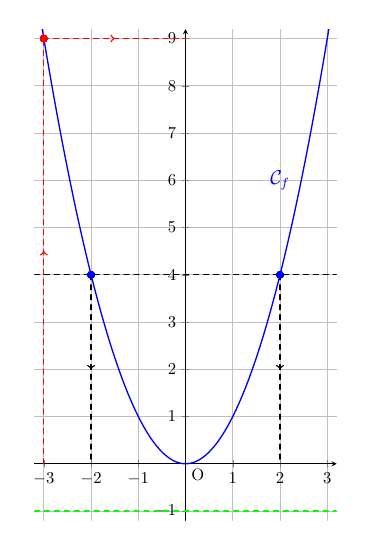
\begin{tikzpicture}[line cap=round,line join=round, x=1.0cm,y=1.0cm,scale=.6]
    \begin{axis}[x=1.0cm,y=1.0cm,axis lines=middle,ymajorgrids=true,xmajorgrids=true,
        xmin=-3.2,xmax=3.2,ymin=-1.2,ymax=9.2,xtick={-3.0,...,3.0},ytick={-1,0,...,9.0},]
        \addplot[thick,blue,domain=-3.2:3.2, samples=100] {x^2};
        \node[below right] at (axis cs:0,0) {O};
        \node[color=blue] at (axis cs:2,6) {\large{$\mathcal{C}_f$}};

        \draw[thick, dashed, green] (axis cs:-3.2,-1) -- (axis cs:3.2,-1);

        \draw[thick, dashed] (axis cs:-3.2,4) -- (axis cs:3.2,4);

\begin{scope}[thick, dashed, decoration={
    markings,
    mark=at position 0.5 with {\arrow{>}}}
    ]
\draw[postaction={decorate}] (axis cs:2,4) -- (axis cs:2,0);
\draw[postaction={decorate}] (axis cs:-2,4) -- (axis cs:-2,0);
\draw[postaction={decorate}, red] (axis cs:-3,0) -- (axis cs:-3,9);
\draw[postaction={decorate}, red] (axis cs:-3,9) -- (axis cs:0,9);
\end{scope}
 %
    \addplot [red, only marks] (-3,9);
    \addplot [blue, only marks] (2,4);
    \addplot [blue, only marks] (-2,4);

    \end{axis}
    \end{tikzpicture}

    \end{center}

        \end{minipage}
        \begin{minipage}{0.45\linewidth}

            \begin{itemize}
                \item
                On lit graphiquement que $f(x)=9$ est l'image de $x=-3$.
                \item
                On lit graphiquement que $-1$ n'a pas d'antécédents.
                \item
                On lit graphiquement que $y=4$ nadmet deux antécédents à savoir $x_1=2$ et $x_2=-2$.
            \end{itemize}

        \end{minipage}

\end{ex}

\section{Résolutions graphique d'équations et d'inéquations}

\end{document}